%#!ptex2pdf -l -u -ot '--synctex=1 --shell-escape' template
%\documentclass[platex]{jsarticle}
\documentclass[platex]{jreport}
% \usepackage[platex]{jreport}
\usepackage{booktabs}
\usepackage{amsmath}
\usepackage{amssymb} 
\usepackage{psfrag}
\usepackage[T1]{fontenc }
\usepackage{pifont}
\usepackage{algorithm}
\usepackage{algorithmic}
\usepackage{amsmath,cases}
\usepackage{here}
\usepackage[dvipdfmx]{graphicx}
\usepackage{url}      %URLの表記に使う\urlコマンドに必要.
\usepackage{enumerate}%enumerate環境で項目を[Step 1.]のような形式に変更するのに利用.
\usepackage{setspace}


\setlength{\topmargin}{-10mm}
\setlength{\textheight}{23cm}
\setlength{\oddsidemargin}{5mm}
\setlength{\evensidemargin}{5mm}
\setlength{\textwidth}{15cm}

\renewcommand{\tablename}{表}
\renewcommand{\figurename}{図}
%\newcommand{\bs}{\texttt{\symbol{'134}}}
%    \newcommand{\cmd}[1]{\texttt{\def\{{\char`\{}\def\}{\char`\}}\bs#1}}
\newtheorem{thm}{定理}[section]
\newtheorem{prf}{証明}[section]
\usepackage{latexsym}
\def\qed{\hfill $\Box$}

\usepackage[margin=3.25cm]{geometry}
\renewcommand{\bibname}{参考文献}

\begin{document}





%%%%%%%%%%%%%%%%%%%%%%%%%%%%%%%%%%%%%%%%%%%%%%%%%
%表紙
\begin{table}[b]
\begin{center}
{\huge 卒\hspace{0.1cm} 業\hspace{0.1cm} 論\hspace{0.1cm} 文}\\[2.5cm]
\begin{spacing}{1.5}
	{\huge 自動車運搬船における貨物積載プランニングの車両配置問題に対する構築型解法}\\[6cm]
\end{spacing}
{\huge 101810106\qquad 黒須諒}\\[1cm]
{\huge 名古屋大学情報学部}\\[0.5cm]
{\huge 自然情報学科数理情報系}\\[0.5cm]
{\huge 2022年2月}\\
\end{center}
\end{table} 
%%%%%%%%%%%%%%%%%%%%%%%%%%%%%%%%%%%%%%%%%%%%%%%%%


\thispagestyle{empty} 
\clearpage
\newpage
\pagenumbering{roman}
\setcounter{page}{1}


%%%%%%%%%%%%%%%%%%%%%%%%%%%%%%%%%%%%%%%%%%%%%%%%%
%摘要とabstract
\begin{center}
\begin{spacing}{1.3}
    {\LARGE 自動車運搬船における貨物積載プランニングの\\車両配置計画に対する構築型解法}\\[0.5cm]
\end{spacing}
\end{center}
\hfill
{\large 101810106\qquad 黒須諒}\\[0.5cm]
\begin{center}
{\Large \bf 概 要}\\
\end{center}

複数の港で自動車を積み, 複数の港で自動車を降ろす自動車運搬船について考える. 
自動車運搬船に積む自動車の集合が与えられてから実際に自動車が船に積まれるまでに, 席割とシミュレーションと呼ばれる二種類の作業が行われる. 
席割作業では, 船の階層内を一定間隔の大きさに区切ったホールドと呼ばれるスペースの各々に, 与えられた積載自動車リストの自動車を何台割り当てられるかを考える. 
シミュレーション作業では席割作業でホールド毎に割り当てられた自動車を, 自動車の向きや空きスペース, 作業効率などを考慮して車一台一台の配置場所を決定する. 
車両配置図を出力することで, 現場の作業員が配置図に従い, 効率よく駐車作業を行うことができる. 
本研究では, シミュレーション作業の自動化を目的とし, 短時間かつ実用的なシミュレーション結果を出力することを目指す. 

シミュレーション作業では車の幅と長さを各辺とした長方形に近似することで, 長方形詰込み問題として定式化することが出来るが, 貨物である自動車は配置位置まで自走するということを考えなければいけない. 
そのため, 積み降ろしのタイミングでは配置場所までの搬入搬出経路の確保と, 駐車時に要する局所的スペースの確保が課題となる. 

本研究では二段階の構築法と局所探索を提案する. 
一段階目では, 積み地, 揚げ地が同じ車を1つのグループとし, デッキ内におけるグループの大まかな配置場所を決定する. 
各グループの積み地, 揚げ地に関する順序対を用意しsequence-pairを用いた制約を追加し, 形状可変の長方形を扱うsoft-rectangleパッキング問題として定式化する. 
以上の定式化により, 搬入搬出時の移動経路を確保した解が得られる. 
この計算には, 商用の整数計画ソルバー(Gurobi Optimizer ver. 9.5)を使用した.  

二段階目では, 第一段階で決められた領域内で車両一台ずつの詳細な配置場所を決定する. 
配置予定の車を, 駐車に必要なスペースを加えたレクトリニア図形に近似し, レクトリニア図形の詰込み問題として定式化する. 
車の向きを考慮したbottom-left法を用いて実装した. 
以上の構築が終わった後, より多くの車を詰め込むために簡単な局所探索を行った.  

以上の提案手法により得られた車両配置図と実際に現場で使われている車両配置図とを比較し, 解の評価を行った. 
その結果, 多くの問題例において, 搬入搬出時の経路確保と駐車時の局所的スペース確保ができていることを確認した. 
また, 構築のみの実装により詰め込むことのできた車の台数と, 局所探索を含めた実装で詰め込むことのできた車の台数を比較した結果, 多くの問題例で局所探索を含めた実装の方がより多くの車を詰め込めることを確認した. 

% 

%%%%%%%%%%%%%%%%%%%%%%%%%%%%%%%%%%%%%%%%%%%%%%%%%%%%%%%
%修士論文の場合は英語のアブストも必要なので以下を記述して下さい
%学位の場合はいらないので, 以下は消して下さい. 
\newpage
\begin{center}{\LARGE A column generation approach \\for the bus crew scheduling problem}\\[0.5cm]
\end{center}
\hfill {\large 351401074\qquad Yuki Sawai}\\[0.5cm]
\begin{center}
{\large \bf Abstract}\\
\end{center}
Write the abstract here.
Unfortunately, if you want a master's degree, you must write the abstract of your master thesis
in English (in addition to the Japanese one) even if you write your thesis in Japanese.
However, if you are going to get a bachelor's degree (not a master's degree),
you don't need to do so.
Good luck!!




\thispagestyle{empty} 
\tableofcontents
\newpage
\setcounter{page}{1}
\pagestyle{plain}
\pagenumbering{arabic}



\chapter{はじめに}

複数の港で自動車を積み, 複数の港で自動車を降ろす自動車運搬船について考える. 
一般的に自動車運搬船は, 自動車を船の一定間隔で区切られたホールドと呼ばれるスペースにどの自動車を何台割り当てるかを決定する席割と呼ばれる工程を経て, 
その後席割作業で割り当てられた自動車に対して向きや場所を考慮して一台ずつ船内の領域に配置するシミュレーションと呼ばれる作業を行う. 
貨物である自動車は積載位置まで自走するため, 積み降ろしのタイミングでの搬入・搬出経路を確保する必要がある. 
また, 航海中の船体バランス及び荷役安全性を考慮する必要がある. 
現状, 自動車を輸送する会社はこの作業を人手で行なっていることが多く, 席割作業に3時間, シミュレーション作業に4時間かかると言われている\cite{mitsui}. 
プランナーごとの経験値や技量によって積み付け計画の品質に個人差が生じ, 急な状況の変化による積み付け計画の変更に業務負荷が生じるなどの問題が存在している. 

名古屋大学の竹田が席割作業の自動化に関する研究を進めている\cite{takeda}. 
本研究では積み付け計画自動化の次の段階としてシミュレーション作業自動化を目的とし, 短時間で実用的なシミュレーション結果を出力することを目指す.  

本研究で扱うシミュレーション作業の概要について述べる. 
入力として, 各階層の各ホールドにどの種類の車を何台詰め込むかという情報が与えられる. 
この情報をもとにシミュレーション作業を行う. 
シミュレーション作業は, 車の全幅と全長を各辺とする長方形に近似することで長方形詰込み問題として定式化できる. 
本研究では, 二段階に分けた構築法を提案する. 
一段階目では, 各ホールド内に詰め込む車を, 積み地や揚げ地の情報をもとにグループ分けし, グループごとにデッキ内での大まかな配置場所を決める. 
二段階目では, グループ内における車両一台ずつの詳細な配置場所を決定する. 

本稿では, 第2章で問題に対する詳細な設定や, 本研究で扱う自動車運輸航海における専門用語について定義する. 
第3章では, 問題の定式化と定式化に必要な変数や定数の定義を行う. 
第4章と第5章では, 提案手法の説明と解の考察を行う. 

\graphicspath{{./sozai/}}
\chapter{問題定義}\label{definition}

シミュレーション作業は各階層ごとに行う.
各階は4つのホールドと呼ばれる一定の広さで区切られたスペースが存在し, 各ホールドに詰め込む車の情報は決まっている.
本稿では複数種類のある階層の中で, 4つのホールドを持つ単純な階層のデータを用いて行う.


\section{用語定義}
本研究で扱う船の航海等に関する専門用語の定義をする\cite{takeda}.

\begin{itemize}
    \item 席割 \\
    注文一つ一つを船のホールドに割り当てる作業.

    \item シミュレーション \\
    席割で決まった自動車を一台ずつホールド内の領域に貼り付ける作業.

    \item  プランナー \\
    席割やシミュレーションを考える作業者.

    \item  オペレーター\\
    港で自動車をホールドまで運転して積み降ろしをする作業者.

    \item デッキ \\
    船の内部の階層.

    \item ホールド \\
    各デッキ内を一定間隔の領域で仕切られた空間. \\
    本研究では, 各デッキは4つのホールドを持つ.

    \item セグメント \\
    隣接するいくつかのホールドをまとめた空間. \\
    本研究では, ホールド1,2とホールド3,4をまとめたものをそれぞれセグメント1, セグメント2と呼ぶ.

    \item ランプ \\
    上下のデッキに移動するために各デッキの特定ホールドについているスロープ.

    \item 積み地 \\
    注文における自動車を積む港.

    \item 揚げ地 \\
    注文における自動車を降ろす港.

\end{itemize}


\section{入力情報}
本研究で扱う2種類の情報について述べる.

\begin{itemize}
    \item 車体情報 \\
    車の数, 種類, 大きさ, 積み地, 揚げ地, 指定のホールド. \\
    本研究では実際のプランで使われているデータを利用した.
    \item 船体情報 \\
    船体の大きさ, 各階のランプの位置, 船内の障害物の位置や大きさ. \\
    本研究では実際の図面データを元に手入力で行った.

\end{itemize}
入力情報のうち車体情報の例を表\ref{table21}に示す.

\begin{table}[htbp]
    \tabcolsep = 10pt
    % \renewcommand{\arraystretch}{0.7}
    \caption{車体情報の例}
    \label{table21}
    \begin{center}
    \begin{tabular}{rcccrcrr} \hline
    番号 & 車種 & 積み地 & 揚げ地 & 数量 & ホールド & 全幅 & 全長 \\ \hline
    1 & Prius & A港 & E港 & 100 & 1 & 200 & 500 \\
    2 & Prius & A港 & E港 & 100 & 2 & 200 & 500 \\
    3 & Aqua & B港 & F港 & 30 & 2 & 250 & 450 \\
    4 & Carolla & C港 & G港 & 60 & 3 & 180 & 480 \\
    5 & Lexus & C港 & G港 & 40 & 3 & 230 & 510 \\
    6 & Lexus & D港 & H港 & 100 & 4 & 230 & 420 \\
    \hline
    \end{tabular}
    \end{center}
    \end{table}

% \begin{figure}[htbp]
%     \hspace{3cm}
%     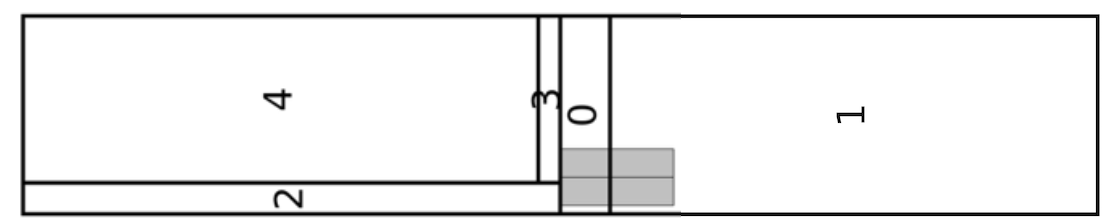
\includegraphics[scale=0.4, bb=0 0 10 10]{2-sennaizu.png}
%     \caption{船内図の例(仮)}
%     \label{figure21}
% \end{figure}


\section{出力}
詰め込むことのできなかった車の台数と配置図を出力する. \\
配置図の例を図\ref{figure22}に示す.
\begin{figure}[b]
    \hspace{2cm}
    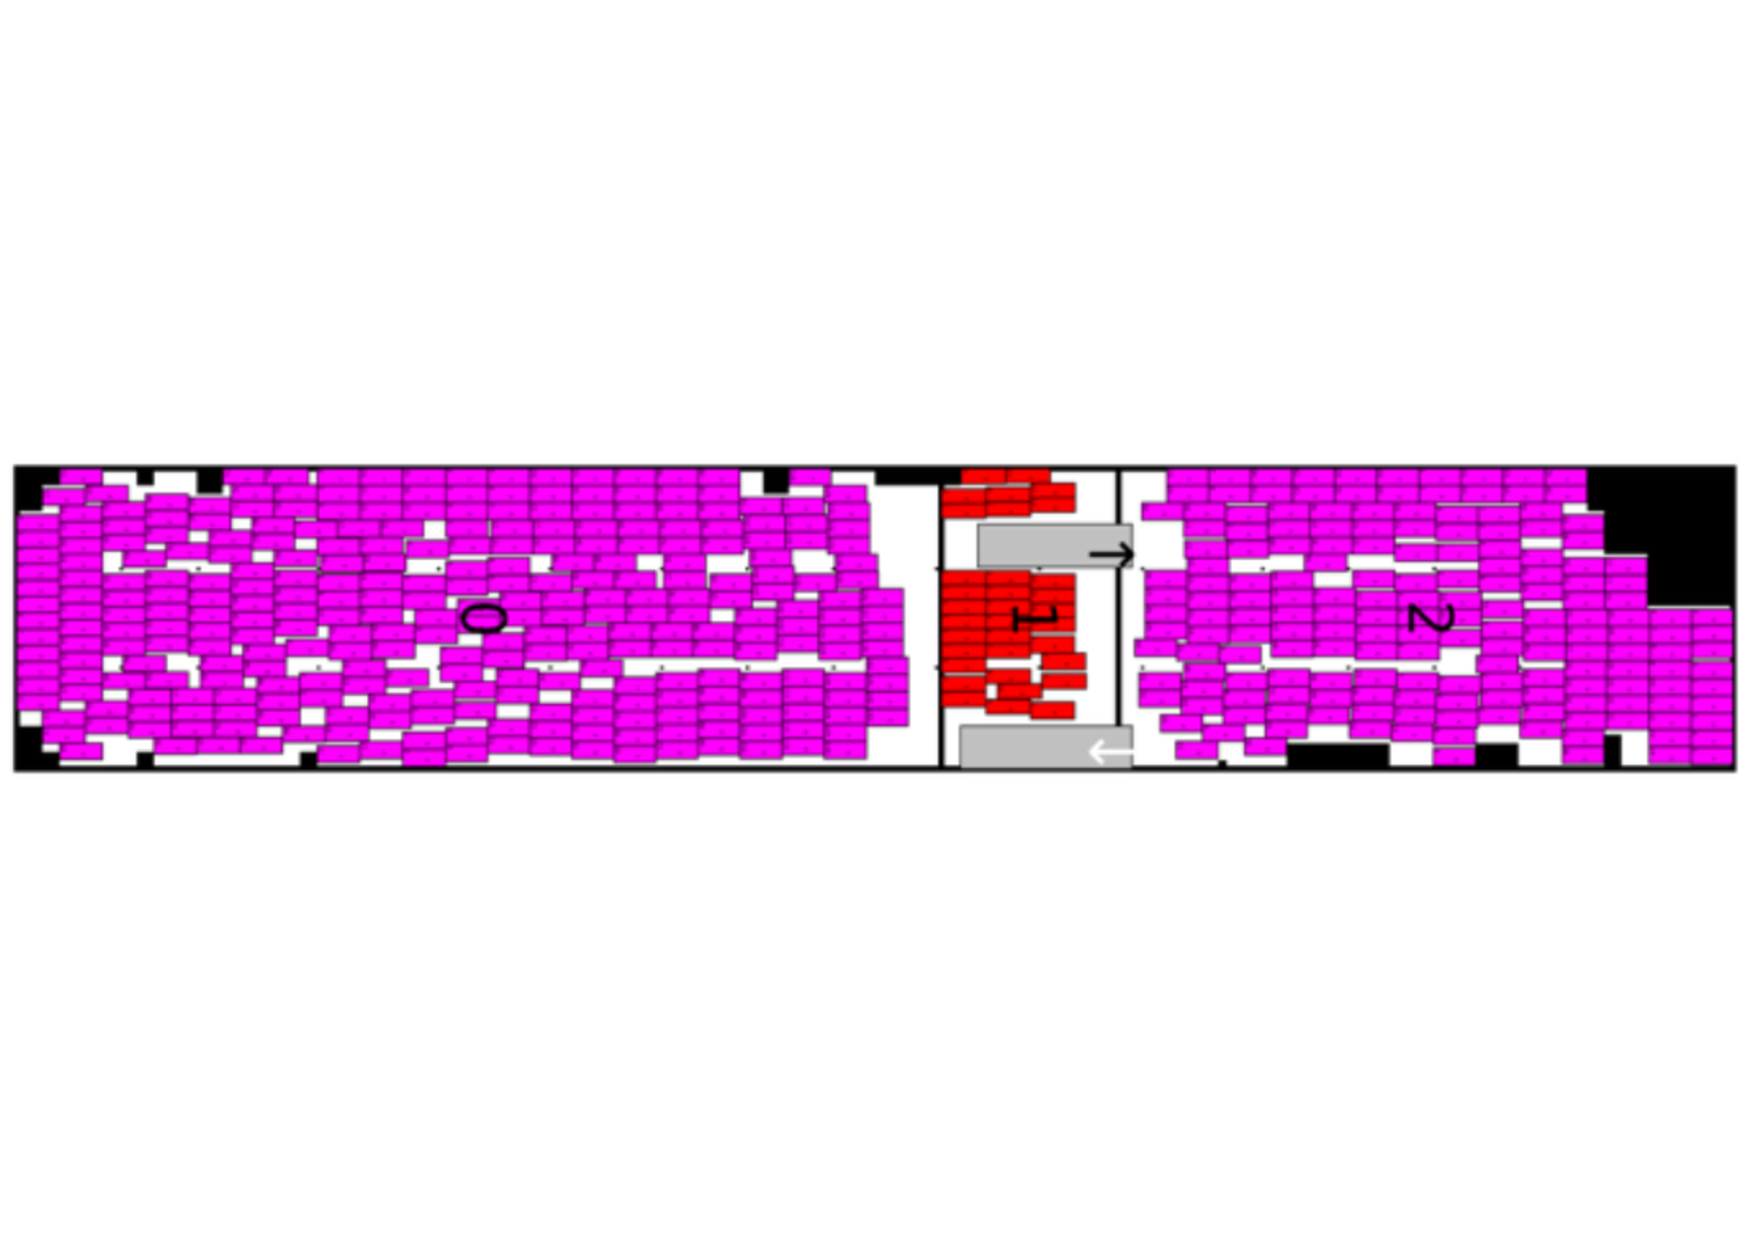
\includegraphics[scale=0.3, bb = 0 0 1 1]{2car_haichi.pdf}
    \caption{車両配置図の例}
    \label{figure22}
\end{figure}


% \begin{table}[htbp]
%     \tabcolsep = 15pt
%     \renewcommand{\arraystretch}{0.8}
%     \caption{出力の例1}
%     \label{table22}
%     \begin{center}
%     \begin{tabular}{rcccrrrr} \hline
%     番号 & 車種 & 積み地 & 揚げ地 & 数量 & ホールド & 横幅 & 高さ \\ \hline
%     1 & Prius & A港 & E港 & 3 & 1 & 200 & 500 \\
%     2 & Prius & A港 & E港 & 5 & 2 & 200 & 500 \\
%     3 & Aqua & B港 & F港 & 10 & 4 & 250 & 450 \\
%     \hline
%     \end{tabular}
%     \end{center}
%     \end{table}

\chapter{定式化}\label{formulation}

この章では1節で本研究における記号の定義や問題の定式化について説明し, 2節では, 本研究に関連する詰込み問題の説明をする. 
その後に, 本問題に関する独自の制約や目的関数を説明し, 定式化する. \\

\section{記号の定義}

\begin{table}[htb]
    \begin{center}
    \label{table31}
    \begin{tabular}{cp{35em}} \hline
    記号 & \hspace{2.0em}記号の説明 \\ \hline

    $x_i$ &
    \begin{tabular}{l}
    \hspace{1.4em}長方形$i$の左下のx座標
    \end{tabular} \\ \hline

    $y_i$ &
    \begin{tabular}{l}
    \hspace{1.4em}長方形$i$の左下のy座標
    \end{tabular} \\ \hline    
    
    $w_i$ &
    \begin{tabular}{l}
    \hspace{1.4em}長方形$i$の幅
    \end{tabular} \\ \hline

    $w_i^l$ &
    \begin{tabular}{l}
    \hspace{1.4em}長方形$i$の幅の下界
    \end{tabular} \\ \hline

    $w_i^u$ &
    \begin{tabular}{l}
    \hspace{1.4em}長方形$i$の幅の上界
    \end{tabular} \\ \hline

    $h_i$ &
    \begin{tabular}{l}
    \hspace{1.4em}長方形$i$の高さ
    \end{tabular} \\ \hline

    $h_i^l$ &
    \begin{tabular}{l}
    \hspace{1.4em}長方形$i$の高さの下界
    \end{tabular} \\ \hline

    $h_i^u$ &
    \begin{tabular}{l}
    \hspace{1.4em}長方形$i$の高さの上界
    \end{tabular} \\ \hline
    
    $W$ &
    \begin{tabular}{l}
    \hspace{1.4em}母材の横幅
    \end{tabular} \\ \hline
    $H$ &
    \begin{tabular}{l}
    \hspace{1.4em}母材の高さ
    \end{tabular} \\ \hline
    $S_i$ &
    \begin{tabular}{l}
    \hspace{1.4em}長方形$i$の面積
    \end{tabular} \\ \hline
    $I$ &
    \begin{tabular}{l}
    \hspace{1.4em}詰め込む長方形の集合
    \end{tabular} \\ \hline
    $\overline{I}$ &
    \begin{tabular}{l}
    \hspace{1.4em}既配置の長方形の集合\ $\overline{I} \subseteq I$
    \end{tabular} \\ \hline
    $J$ &
    \begin{tabular}{l}
    \hspace{1.4em}障害物の集合
    \end{tabular} \\ \hline
    
    
    \end{tabular}
    \end{center}
    \end{table}

\section{一般論(仮タイトル)}

\subsection{長方形詰込み問題}
長方形詰込み問題とは, 母材の幅$W$と高さ$H$, 長方形集合$I$に対し, 幅$w_i$, 高さ$h_i$が入力として与えられ, 母材からはみ出ることなくまた, どの二つの長方形も互いに重なることがないように詰め込む問題である. \\
以上の条件を定式化すると, 次のように書くことができる. \\
\textgt{条件1: 長方形$i \in I$は母材上に配置される. }\\
\begin{eqnarray}
    0 \leq x_i \leq W-w_i \ (i \in I), \\
    0 \leq y_i \leq H-h_i \ (i \in I). 
\end{eqnarray}
\textgt{条件2: 長方形$i,j \in I$は互いに重ならない. }\\
この条件は, 次の4つの不等式のうち一つ以上が成立しなければいけない.  
\begin{eqnarray}
    x_i + w_i \leq x_j \ (i \in I), \\
    x_j + w_j \leq x_i \ (i \in I), \\
    y_i + h_i \leq y_j \ (i \in I), \\
    y_j + h_j \leq y_i \ (i \in I). 
\end{eqnarray}

\subsection{Soft-rectangleパッキング問題}
長方形詰込み問題の一種で, 詰め込む長方形の幅と高さを可変としたsoft-rectangle (可変形状長方形)を扱う\cite{soft-rectangle}. 
長方形の座標$x,y$だけでなく幅$w$と高さ$h$も変数とする. \\
通常, 長方形$i \in I$の面積に関する次のような等式制約または不等式制約が存在する: \\
\begin{eqnarray}
    w_i * h_i = S_i, \\
    w_i * h_i \geq S_i. \\
\end{eqnarray}
また, 長方形 $i \in I$の幅と高さの上界, 下界に関する以下の制約も存在する: 
\begin{eqnarray}
    w_i^l \leq w_i \leq w_i^u, \\
    h_i^l \leq h_i \leq h_i^u. 
\end{eqnarray}

\subsection{Sequence-pair}
Sequence-pairとは, 二つの順列による長方形の配置表現である\cite{seq-pair}. 
長方形同士の相対位置関係を長方形名の順列対により表すことができる. 
例を図\ref{s-p-eg}に示す. 制約の詳細は3.3節で説明する. 
Sequence-pairはどのような配置表現でも一意の順列対に表現でき, 逆に任意の順列対から一意に配置表現を求めることができる. \\ 

\begin{figure}[b]
    \hspace{2cm}
    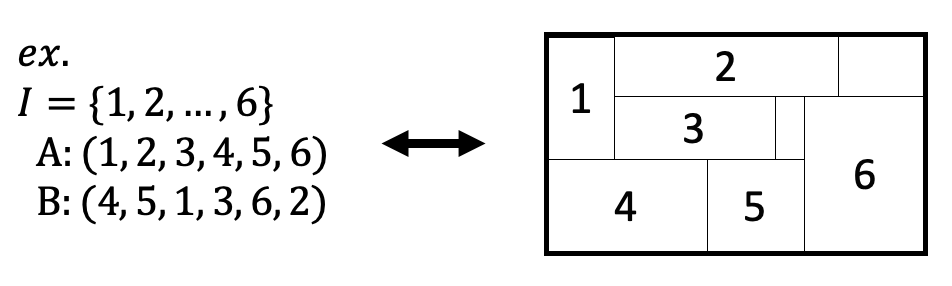
\includegraphics[scale=0.3, bb = 0 0 1 1]{3-sequence-pair.png}
    \caption{sequence-pairによる長方形配置表現}
    \label{s-p-eg}
\end{figure}
\clearpage

\subsection{No-fit polygon}
No-fit polygon (NFP)とは, 平面上で多角形の重なりを判定する方法である\cite{nfp}\cite{nfp2}. 
多角形$P$と$Q$が与えられ, $Q$の配置が固定されているとする. 
この時, 多角形$P$が$Q$と重なりを持つ領域をNFP($P,Q$)と書き, 図\ref{nfp-eg}に示す. 
図\ref{nfp-eg}の太線がNFPの境界を表し, このNFP内に$P$を配置すると$Q$と重なることを意味する. 
母材内の既配置の長方形全てに対し, 長方形$i$のNFPを作成すると, 長方形$i$の配置可能領域はどのNFPの内部にも含まれない領域である. \\


\begin{figure}[tbp]
    \hspace{3cm}
    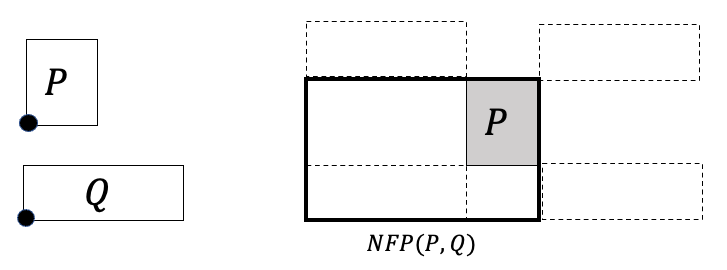
\includegraphics[scale = 0.3, bb=0 0 10 10]{3nfp.png}
    \caption{NFP($P,Q$)}
    \label{nfp-eg}
\end{figure}

\section{第一段階}
第一段階では, 積み地・揚げ地が同じ車を一つのグループとし, 各グループのデッキ内における大まかな配置場所を決定する. 
グループ内の車の総面積を計算し, soft-rectangleパッキング問題として定式化する. 
このパッキングはセグメントごとに行う. 

\subsection{制約}
\textgt{(i)ランプから配置場所までの移動経路確保に関する制約}\\
\ プランナーへのヒアリングの結果から, 先に積む貨物ほど入口から見て奥に積み, 後から積む貨物ほど手前に積むことが望ましいと分かった. 
同様に, 先に降ろす貨物ほど入口から見て手前に積み, 後から下ろす荷物ほど奥に積むこともまた望まれる. 
本研究では, Sequence-pairを用いてグループの相対位置関係に関する制約を表現する. 
各グループを積み地の昇順に並べた順列を$\sigma^+$とする. 
積み地が同じグループが存在した場合, 揚げ地の降順に従う. 
同様に, 揚げ地の降順に並べた順列を$\sigma^-$とする.
揚げ地が同じグループが存在する場合, 積み地の昇順に従う. \\
グループの集合を$I$とし, グループ$i,j \in I$に関して, 順序対$(\sigma^+,\sigma^-)$における$i,j$の順序関係をもとに, 以下のどちらかの制約を追加する: \\
\begin{eqnarray}
    \left\{
        \begin{array}{ll}
            y_i + h_i \leq y_j & \sigma^+(\ldots,i,\ldots,j,\ldots) \cap \sigma^-(\ldots,i,\ldots,j,\ldots) \\
            x_i + w_i \leq x_j & \sigma^+(\ldots,i,\ldots,j,\ldots) \cap \sigma^-(\ldots,j,\ldots,i,\ldots) \\
        \end{array}
    \right.
\end{eqnarray}\\


\textgt{(ii)各グループの面積に関する制約}\\
\ 次の段階で各グループの車を詰め込むためには, グループの面積はグループ内に属する車の総面積よりも大きくなければいけない. 
以上の制約は, グループの集合を$I$とし, グループ$i \in I$の車の総面積を$S_i$とすると, 以下のように書ける: \\
\begin{eqnarray}
    w_i*h_i \geq S_i , 
\end{eqnarray}
一つのグループの領域が大きくなりすぎると, デッドスペースが生まれたり, 他のグループの領域で詰め込めない車が出てしまう可能性があるので, パラメータ変数$a (a \geq 1)$を用意して, 以下のように上から抑える. 
\begin{eqnarray}
    w_i*h_i \leq a*S_i.
    \label{a_const}
\end{eqnarray}\\

\textgt{(iii)各グループの幅と高さに関する制約}\\
\ 各グループ$I$の幅と高さは, グループ内に属する車$i \in I$の幅と全長の最大値をもとに以下の下限を設定する: \\
\begin{eqnarray}
    w_I \geq \max_{i \in I} w_i, \\
    h_I \geq \max_{i \in I} h_i. 
\end{eqnarray}


\subsection{目的関数}
目的関数として, デッキ内のより多くの領域を配置可能場所として使えることが望ましいので, グループの面積和の最大化を目指す. 
また1つのグループが大きくなりすぎると, デッドスペースが生まれたり, 他のグループの領域で詰め込めない車が出てしまう可能性があるので, バランス良く大きくすることを目指す. 
面積制約\ref{a_const}で用いたパラメータ$a$を用いて, 以下のように書くことができる: \\
\begin{eqnarray}
    \mathrm{maximize}\ \sum_{i \in I} w_i*h_i  - a. 
\end{eqnarray}
\subsection{定式化}
パッキングするグループの集合を$I$とし, セグメントの幅と高さをそれぞれ$W, H$とし, 以上をまとめると以下のようになる. \\
\begin{center}
    \begin{align}
        & \textrm{maximize} \hspace{1.5cm}
        \sum_{i \in I} w_i - h_i - a \\
        & \textrm{subject\ to} \hspace{1.5cm}
        0 \leq x_i \leq W - w_i & (i \in I) \\
        &\hspace{3cm} 0 \leq y_i \leq H - y_i & (i \in I) \\
        &\hspace{3cm} 0 \leq w_i \leq \max_{car \in i}w_{car} & (i \in I) \\
        &\hspace{3cm} 0 \leq h_i \leq \max_{car \in i}h_{car} & (i \in I) \\
        &\hspace{2.8cm} S_i \leq w_i*h_i \leq a*S_i &(i \in I)
    \end{align}
    \begin{eqnarray}
        \hspace{2cm} \left\{
            \begin{array}{ll}
                y_i + h_i \leq y_j & \sigma^+(\ldots,i,\ldots,j,\ldots) \cap \sigma^-(\ldots,i,\ldots,j,\ldots) \\
                x_i + w_i \leq x_j & \sigma^+(\ldots,i,\ldots,j,\ldots) \cap \sigma^-(\ldots,j,\ldots,i,\ldots) \\
            \end{array}
        \hspace{2cm} \right.
    \end{eqnarray}
\end{center}

\section{第二段階}
第二段階では, 第一段階で決められた領域をはみ出ることがないように, 車一台ずつの配置場所を決定する. 
車を長方形に近似することで, 長方形詰込み問題として定式化する. 

\subsection{制約}
\textgt{(i)駐車に必要な局所的なスペースに関する制約}\\
\ 駐車は原則バック駐車で行うため, 配置位置周辺に局所的なスペースが必要となる. 
例えば, 配置位置のすぐ前方に柱等の障害物があると, 配置図上では配置可能に見えても, 実際には障害物が邪魔で駐車できない可能性がある.
この点を考慮するため, 予め駐車に必要なスペースを定義する.
プランナーへのヒアリングの結果から, 駐車にはおおよそ車体長さの半分に相当するスペースが必要で, このスペース上に障害物がなければ良いということが分かった. 
車$i$の大きさと駐車に必要なスペースを合わせたレクトリニア図形を$f(i)$で定義する. 
障害物の集合を$J$, 既配置の車の集合を$\overline{I}$とすると, 車$i$の配置不可能な領域はNFPの表現を用いて以下のように書くことができる.  
\begin{eqnarray}
    \label{nfp-eq1}
    \sum_{j \in J} NFP(f(i),j) + \sum_{\overline{i} \in \overline{I}} NFP(f(i),\overline{i})
\end{eqnarray}\\

\textgt{(ii)配置間隔に関する制約}\\
配置される車の間隔は他の車両や障害物と前後方向に10cm, 左右方向に40cm空いている必要がある. 
先ほどの制約同様, 配置予定の車を上記の単位だけ大きくしてNFPを計算する. 
車両$i$を上下方向に10cmずつ, 左右方向に40cmずつ大きくした長方形を$g(i)$とすると, 車両$i$の配置不可能な領域は以下のように表される. 
\begin{eqnarray}
    \label{nfp-eq2}
    \sum_{j \in J} NFP(g(i),j) + \sum_{\overline{i} \in \overline{I}} NFP(g(i),\overline{i})
\end{eqnarray}

車両$i$が配置可能な領域は, (\ref{nfp-eq1}), (\ref{nfp-eq2})以外の領域である. 

\subsection{目的関数}
第二段階では, 目的関数の設定は行わず解の構築のみを行う. 

\subsection{定式化}
まとめると, グループ$I$内の車$i$をパッキングする時の制約は, 以下のようになる. 
\begin{center}  
\begin{align}
    & \textrm{subject\ to} \hspace{1cm}0 \leq x_i \leq W_I - w_i & (i \in I)\\
    & \hspace{2.6cm} 0 \leq y_i \leq H_I - h_i & (i \in I)\\
    & \hspace{2.6cm} x_i + w_i \leq x_j \hspace{0.3cm}or\hspace{0.3cm} x_j + w_j \leq x_i \hspace{0.3cm}or \nonumber \\
    & \hspace{2.6cm} y_i + h_i \leq y_j \hspace{0.3cm}or\hspace{0.3cm} y_j + h_j \leq y_i &(i,j \in I)\\
    & \hspace{2cm} (x_i, y_i) \neq \sum_{j \in J} NFP(f(i)+g(i),j) + \sum_{\overline{i} \in \overline{I}}NFP(f(i)+g(i),\overline{i}) & (i \in I)
\end{align}
\end{center}
\chapter{提案手法}\label{method}
本章では, 第3章で定式化した二段階の問題についてそれぞれの問題に対する提案手法を説明する. 

\section{第一段階}
求解には整数計画ソルバー (Gurobi Optimizer ver. 9.5)を用いた. 
第二段階では, この時の出力結果を利用しする.  

\section{第二段階}
\subsection*{bottom-left法}
bottom-left法 (BL法)とは長方形詰込み問題に対するアルゴリズムの一つで, 配置可能な領域の内, 最も下に, 同じ高さの候補があれば, 最も左に配置する手法である\cite{nfp2}. 
面積の大きい順にパッキングするといったように, 詰め込む順番を工夫することで有用な解が得られるとされている. \\


本研究では, 車の駐車向きを考慮し, 駐車後にランプを向かって前向きに発進できるようにBL法を修正し, 詰め込みを行った. 
各グループ内で, 高さの低いもの, その中でも幅の小さいものを先に, そして同じ車種が連続するような順番で詰め込みを行った. 
グループ間の詰め込みの順番としては, 積み地の早い順, 積み地が同じ場合, 揚げ地の遅い順に詰め込みを行った. 

グループ内の全ての車が詰め終わるか, 詰め込み途中で, グループ内のどの車も詰め込むことができない場合, 計算を終了し, 次のグループ内の車の詰め込みを開始した. 

% \chapter{提案手法2}\label{method2}

\chapter{計算実験}\label{computational_result}
\section{計算環境}
実験に用いるプログラムはPythonを用いて実装し, 計算機はMacBookAir(CPU: Apple M1 chip, メモリ: 8GB)を用いて行った. 

\section{第一段階の求解結果}
整数計画ソルバー (Gurobi Optimizer ver. 9.5)を用いて計算した結果, 全ての問題例で最適解が得られた. 
出力の例を図\ref{first-no-rei}に示す. 
長方形内の番号はグループの番号を表す. 
灰色の長方形は, ランプを表す. \\

\begin{figure}[b]
    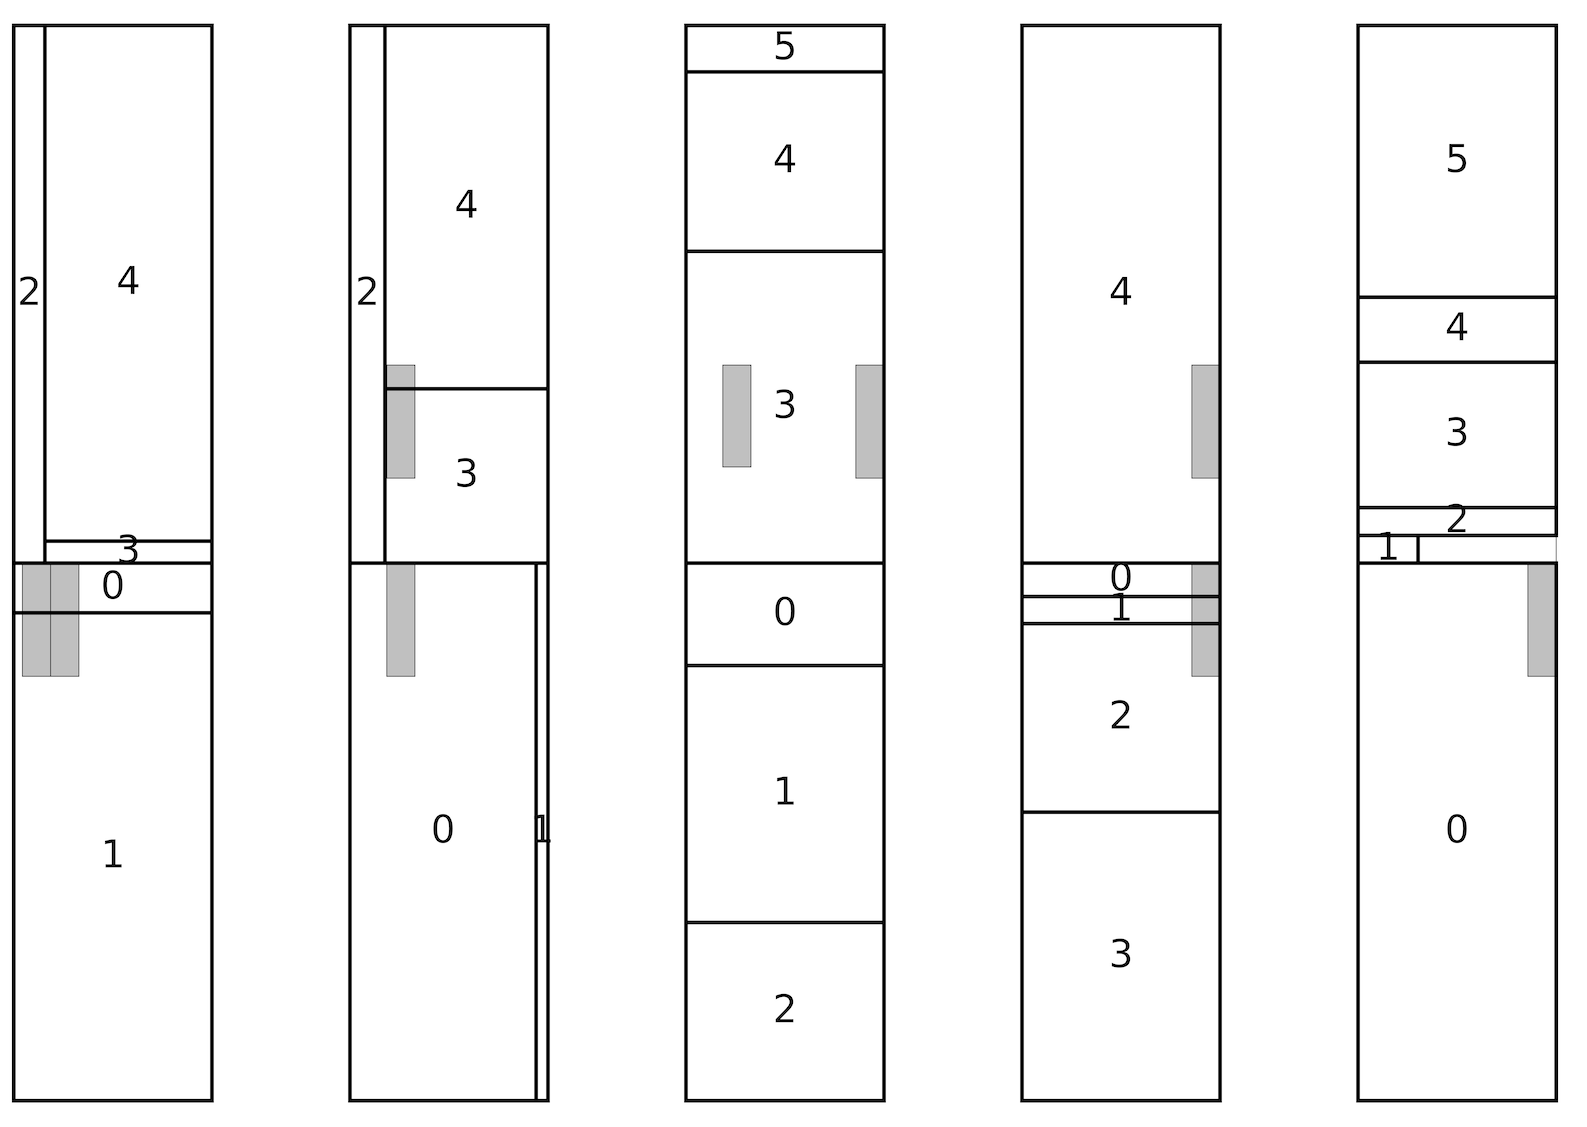
\includegraphics[scale=0.3, bb = 0 0 1 1]{5-first-no-rei.png}
    \caption{第一段階の出力の例}
    \label{first-no-rei}
\end{figure}
\clearpage

\section{第二段階の求解結果}
出力される配置図を図\ref{second-no-rei}に示す. 
各長方形が車を表し, 色は積み地の種類を表す. \\

\begin{figure}[b]
    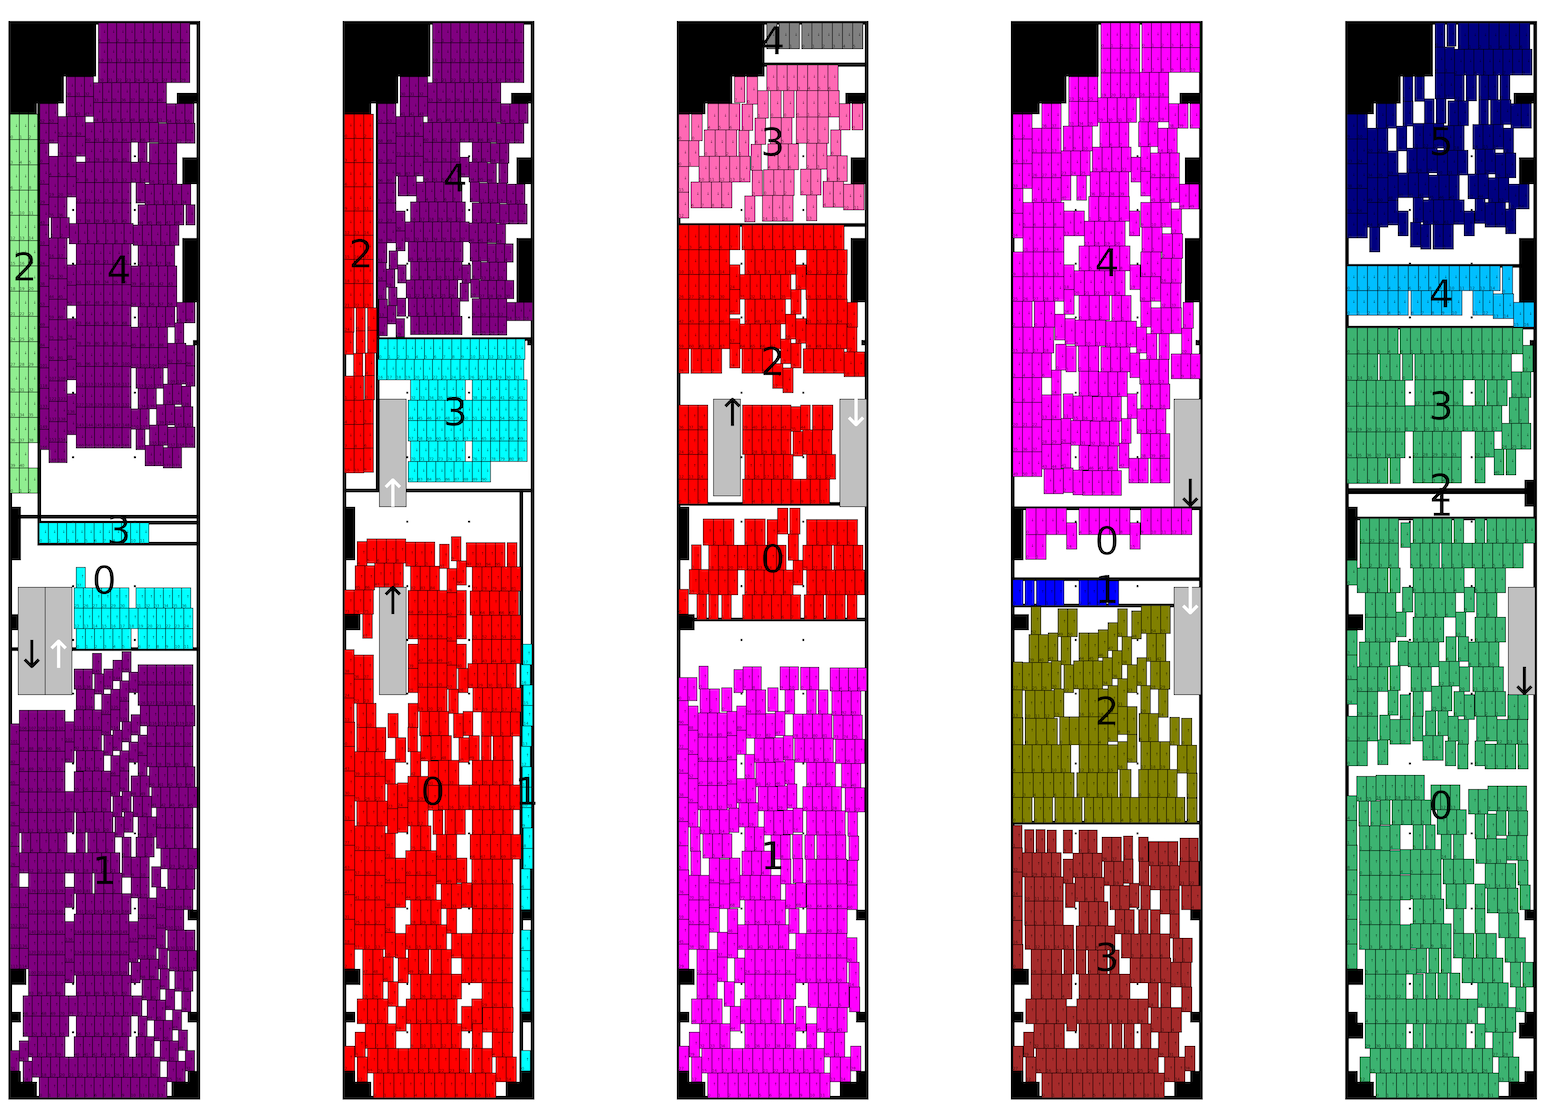
\includegraphics[scale=0.3, bb = 0 0 1 1]{5-second-no-rei.png}
    \caption{第一段階の出力の例}
    \label{second-no-rei}
\end{figure}


\chapter{まとめと今後の研究計画}\label{conclution}
自動車運搬船への貨物積み付け計画における,車両配置計画に対して2段階の構築法を提案した.
2段階にすることで,各車の積み地と揚げ地における導線確保と駐車時の局所的スペース確保を実現した.
1段階目では,シーケンスペアとsoft-rectangleパッキング問題に帰着することで求解することができた.
2段階目では,レクトリニア図形とパッキング問題に有用なbottom-left法を用いて構築した.

\chapter*{謝辞}
本研究の遂行にあたり, 熱心な指導と助言を頂きました柳浦睦憲教授に深く感謝の意を表します. 
提案手法の検討やその有用性において活発に議論を頂きました, 胡艶楠氏, 竹田陽氏には大変お世話になりました. 深くお礼申し上げます. 
日々の研究室生活においては柳浦研究室の皆様にお世話になりました. 
皆様のおかげで有意義な研究活動に勤しむことができました. 深くお礼申し上げます. 




\addcontentsline{toc}{chapter}{参考文献}
\begin{thebibliography}{99}
	\bibitem{mitsui}
	「商船三井 プレスリリース」https://www.mol.co.jp/pr/2019/19072.html (2022年1月26日)
	\bibitem{rect-pack}
	今堀慎治, 梅谷俊治, "切り出し・詰込み問題とその応用 -- (2) 長方形詰込み問題--," オペレーションズ・リサーチ, 50, (2005), 335--340
	\bibitem{soft-rectangle}
	T. Ibaraki and K. Nakamura, "Packing Problems with Soft Rectangles," LNCS 4030, (2006), 13--27
	\bibitem{seq-pair}
	H. Murata, K. Fujiyoshi, S. Nakatake and Y. Kajitani, "VLSI Module Placement Based on Rectangle-Packing by the Sequence-Pair," 
	IEEE Transactions on Computer-aided Design of Integrated Circuits and Systems, 15(12):1518--1524, December 1996.
	\bibitem{nfp}
	R. C. Art, "An approach to the two dimensional irregular cutting stock problem,"
	Ph.D. Thesis, Massachusetts Institute of Technology, 1966.
	\bibitem{nfp2}
	今堀慎治, 胡艶楠, 橋本英樹, 柳浦睦憲, "Pythonによる図形詰込みアルゴリズム入門," 
	オペレーションズ・リサーチ, (2008), 762--769
	\bibitem{takeda}
	竹田陽, "自動車運搬船における貨物積載プランニングの席割問題に対する局所探索," 修士論文, 名古屋大学情報学研究科, 2022


\end{thebibliography}
\end{document}



% LocalWords:  ij Imahori Yagiura Ibaraki th Metaheuristics McGeoch Aarts lrr
% LocalWords:  Lenstra Chichester algorithmicx Fulkerson lrrcrr
%%presented by YUKI SAWAI 2015/12/22
%この卒論修論はhttp://www.co.cm.is.nagoya-u.ac.jp/~yagiura/writing/haifu_template/をもとに澤井佑樹が作っています
